\documentclass[12pt,titlepage]{article}
\usepackage[margin=1.25in]{geometry}
\usepackage{graphicx,amsmath,blindtext}

%% Variables definition
\newcommand{\vSubject}{Statistical Computations}
\newcommand{\vSubtitle}{Quiz 1}
\newcommand{\vName}{Dicha Zelianivan Arkana}
\newcommand{\vNIM}{2241720002}
\newcommand{\vClass}{2i}
\newcommand{\vDepartment}{Information Technology}
\newcommand{\vStudyProgram}{D4 Informatics Engineering}

%% [START] Tikz related stuff
\usepackage{tikz}
\usetikzlibrary{svg.path,calc,shapes.geometric,shapes.misc}
\tikzstyle{terminator} = [rectangle, draw, text centered, rounded corners = 1em, minimum height=2em]
\tikzstyle{preparation} = [chamfered rectangle, chamfered rectangle sep=0.75em, draw, text centered, minimum height = 2em]
\tikzstyle{process} = [rectangle, draw, text centered, minimum height=2em]
\tikzstyle{decision} = [diamond, aspect=2, draw, text centered, minimum height=2em]
\tikzstyle{data}=[trapezium, draw, text centered, trapezium left angle=60, trapezium right angle=120, minimum height=2em]
\tikzstyle{connector} = [line width=0.25mm,->]
%% [END] Tikz related stuff

%% [START] Fancy header related stuff
\usepackage{fancyhdr}
\pagestyle{fancy}
\setlength{\headheight}{15pt} % compensate fancyhdr style
\fancyhead{}
\fancyfoot{}
\fancyfoot[L]{\thepage}
\fancyfoot[R]{\textit{\vSubject - \vSubtitle}}
\renewcommand{\footrulewidth}{0.4pt}% default is 0pt, overline for footer
%% [END] Fancy header related stuff

%% [START] Custom tabular command related stuff
\usepackage{tabularx}
\newcommand{\details}[2]{
    #1 & #2  \\
}
%% [END] Custom tabular command related stuff

%% [START] Figure related stuff
\newcommand{\image}[3][1]{
    \begin{figure}[h]
        \centering
        \includegraphics[#1]{#2}
        \caption{#3}
        \label{#3}
    \end{figure}
}
%% [END] Figure related stuff

\begin{document}
\begin{titlepage}
    \centering
    \vfill
    {\bfseries\LARGE
        \vSubject\\
        \vskip0.25cm
        \vSubtitle
    }
    \vfill
    
\includegraphics[width=6cm]{images/polinema-logo.png}
    \vfill
    {
        \textbf{Name}\\
        \vName\\
        \vskip0.5cm
        \textbf{NIM}\\
        \vNIM\\
        \vskip0.5cm
        \textbf{Class}\\
        \vClass\\
        \vskip0.5cm
        \textbf{Department}\\
        \vDepartment\\
        \vskip0.5cm
        \textbf{Study Program}\\
        \vStudyProgram
    }
\end{titlepage}

\section{Question 1}

Terdapat data status gizi balita di Kota Magelang Berdasarkan Kecamatan dan Jenis Kelamin.
Dari data tesebut, diketahui bahwa terdapat 4 kategori pengelompokan gizi, yaitu:
\begin{enumerate}
    \item Gizi sangat kurang
    \item Gizi kurang
    \item Gizi baik
    \item Gizi lebih
\end{enumerate}

\begin{enumerate}
    \item {
        Berdasarkan file tersebut, jelaskan terdapat data apa saja dan tipe data masing-masing sata.
        \begin{itemize}
            \item \textbf{Kecamatan / Kelurahan} - Kualitatif - Nominal
            \item \textbf{Balita Ditimbang Laki Laki} - Kuantitatif - Diskrit
            \item \textbf{Balita Ditimbang Perempuan} - Kuantitatif - Diskrit
            \item \textbf{Status Gizi Baik Laki - Laki} - Kuantitatif - Diskrit
            \item \textbf{Status Gizi Baik Perempuan} - Kuantitatif - Diskrit
            \item \textbf{Status Gizi Kurang Laki - Laki} - Kuantitatif - Diskrit
            \item \textbf{Status Gizi Kurang Perempuan} - Kuantitatif - Diskrit
            \item \textbf{Status Gizi Sangat Kurang Laki - Laki} - Kuantitatif - Diskrit
            \item \textbf{Status Gizi Sangat Kurang Perempuan} - Kuantitatif - Diskrit
            \item \textbf{Status Gizi Lebih Laki - Laki} - Kuantitatif - Diskrit
            \item \textbf{Status Gizi Lebih Perempuan} - Kuantitatif - Diskrit
        \end{itemize}
    }
    \item {
        Data gizi balita tersebut apakah dapat dikategorikan sebagai one-way data ataukah two-way data? Jelaskan alasannya.

        The data is one way data because it only has one variable, which is the status of the children that relates to the kecamatan
    }
    \item {
        Tampilkan dalam bentuk grafik, total keseluruhan balita yang sudah di timbang di Kabupaten Magelang. Selanjutnya, tampilkan prosentase bayi laki-laki dan perempuan yang sudah di timbang.

        \begin{center}
            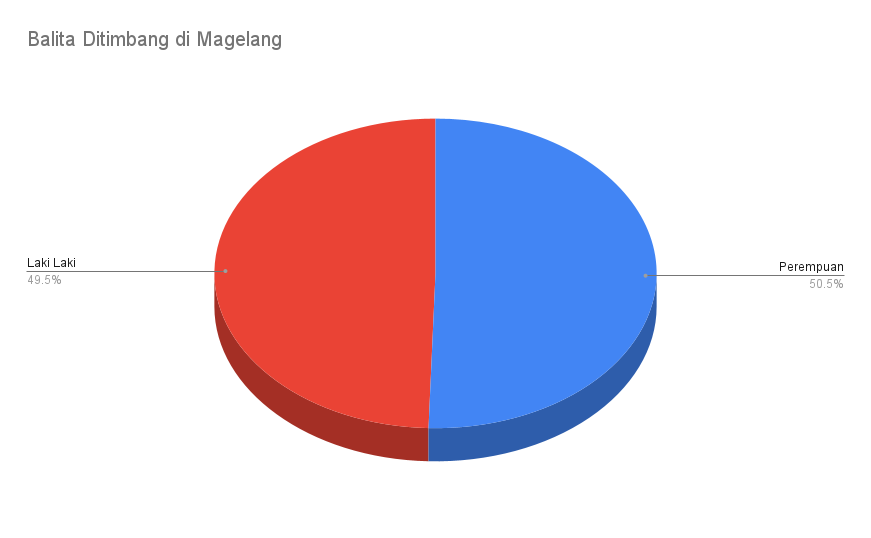
\includegraphics[width=0.9\textwidth]{./images/balita_ditimbang_magelang.png}
        \end{center}
        \begin{center}
            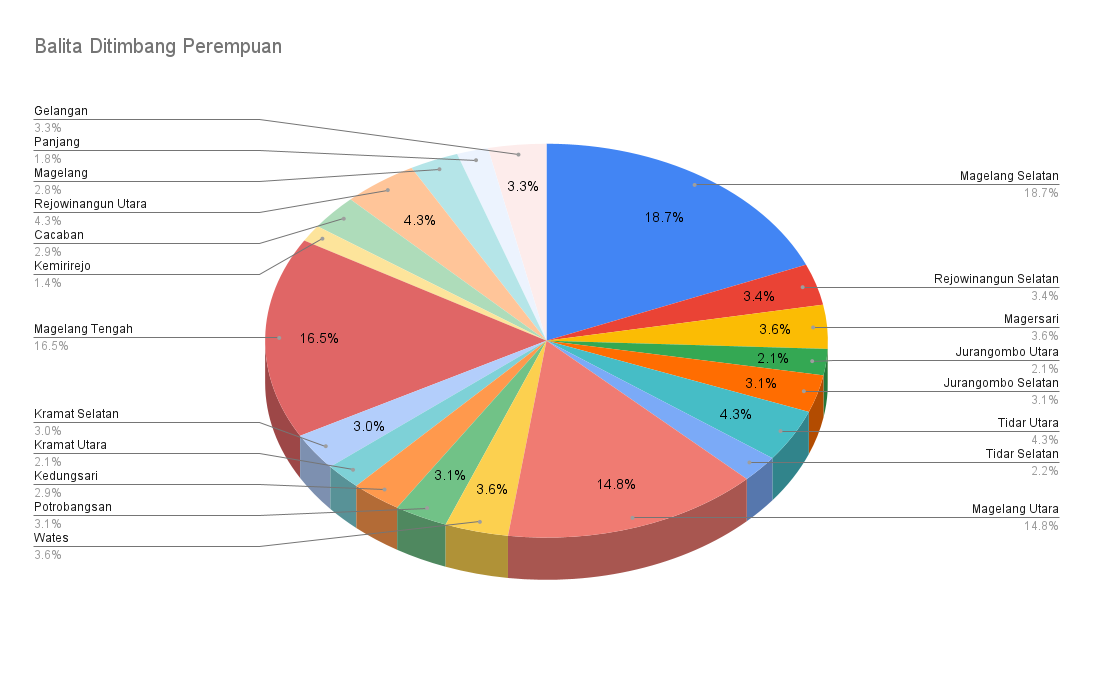
\includegraphics[width=0.9\textwidth]{./images/balita_ditimbang_perempuan.png}
        \end{center}
        \begin{center}
            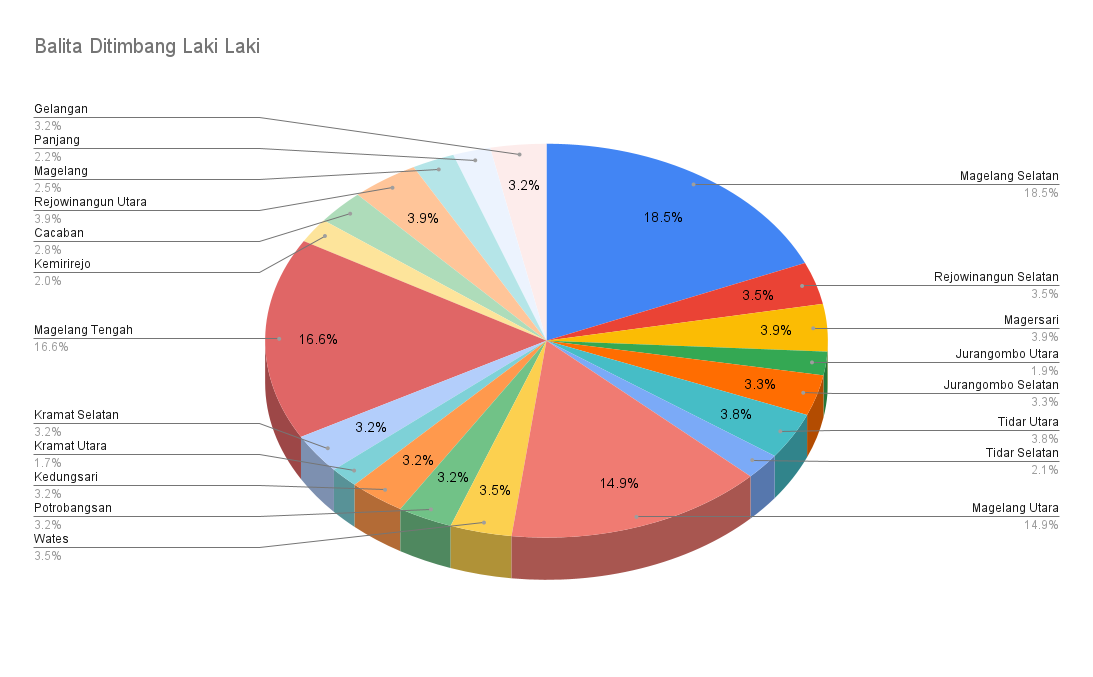
\includegraphics[width=0.9\textwidth]{./images/balita_ditimbang_laki_laki.png}
        \end{center}
    }
    \item {
        Kepada Dinas Kesehatan Kabutapan Magelang ingin mengetahui presentasi data gizi balita untuk setiap kategorinya. Buatlah presentasi data yang sesuai dengan permintaan tersebut.

        \begin{center}
            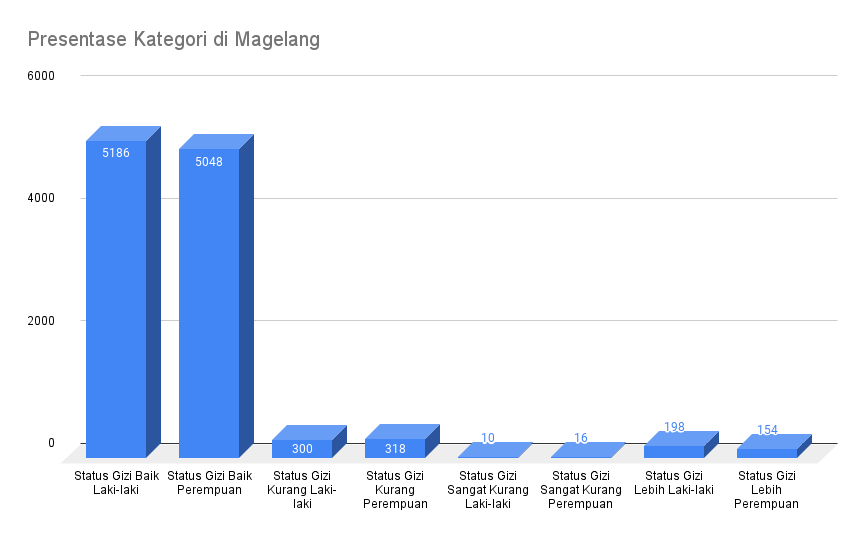
\includegraphics[width=0.9\textwidth]{./images/presentasi_kategori_magelang.png}
        \end{center}
    }
    \pagebreak
    \item {
        Bupati Magelang ingin membuat kebijakan terkait dengan bantuan untuk \\menginkatkan gizi balita.
        Oleh karena itu, Bupati harus mengetahui jumlah balita untuk setiap ketegori di semua kecamatan di Kabupaten Magelang.
        Data ini akan sangat berguna untuk memprioritaskan bantuan nantinya. Untuk mempermudah Bupati, presentasi apa yang dapat ditampilkan?

        \begin{center}
            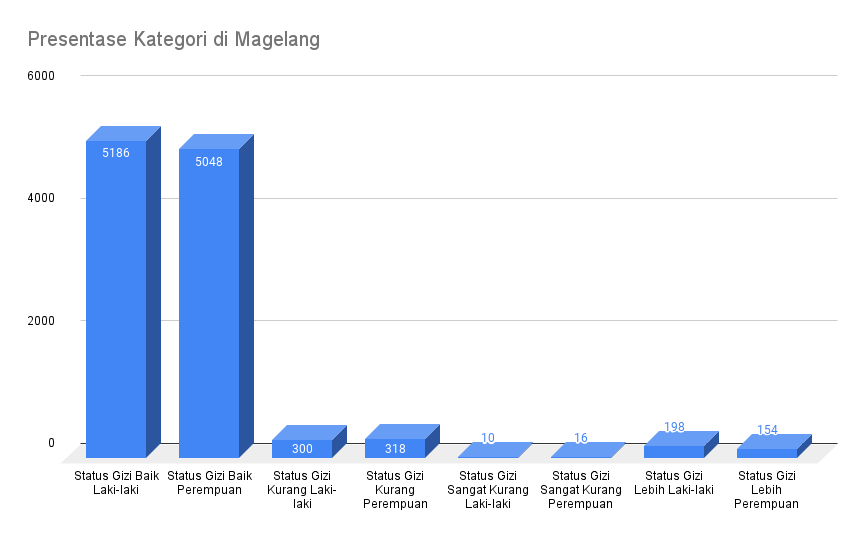
\includegraphics[width=0.9\textwidth]{./images/presentasi_kategori_magelang.png}
        \end{center}
    }
\end{enumerate}

\end{document}

